\documentclass[12pt]{article}
\usepackage[a4paper, left=1.5cm, right=1.5cm, top=1.5cm, bottom=1.5cm]{geometry}
\usepackage{emptypage}
\usepackage{bm}
\usepackage{graphicx}
\usepackage[parfill]{parskip}
\usepackage{xfrac}
\usepackage{mathtools}
\usepackage[table]{xcolor}
\usepackage{array}
\newcolumntype{P}[1]{>{\raggedright\arraybackslash}p{#1}}
\usepackage{pdfpages}
\usepackage{enumitem}
\usepackage{mdframed}
\usepackage{setspace}
\usepackage{amsmath}
\usepackage{mathtools}
\usepackage{mathrsfs, amssymb}
\usepackage{layout}
\usepackage{lscape}
\usepackage{booktabs}
\usepackage{multirow}
\usepackage{multicol}
\usepackage{soul}
\usepackage[customcolors,shade]{hf-tikz}
\definecolor{linkcolour}{rgb}{0,0.5,0.5}
\usepackage{hyperref}
\hypersetup{
	colorlinks=true,
	linkcolor=linkcolour,
	filecolor=magenta,      
	urlcolor=linkcolour
}

\usepackage{calc}
\usepackage{tikz}
\usepackage{mdframed}

\definecolor{gold}{HTML}{D4AF37} % correct answer
\definecolor{green}{rgb}{0.55, 0.71, 0.0} % steps to take
\definecolor{orange}{rgb}{0.93, 0.53, 0.18} % derivation / overarching theme
\definecolor{pink}{rgb}{0.87, 0.36, 0.51} % important
\definecolor{blue}{HTML}{0073CF} % concept example
\definecolor{purple}{rgb}{0.6, 0.4, 0.8} % theme of sentence / concept
\definecolor{yellow}{rgb}{0.99, 0.93, 0.0} % definition
\definecolor{red}{rgb}{1.0, 0.11, 0.0} % very important
\definecolor{exblue}{HTML}{00FFEF} % exercise example
\definecolor{lightpurple}{HTML}{D19FE8} % subpoint

\newcommand{\lightpurple}[1]{%
	\begingroup
	\sethlcolor{lightpurple}%
	\hl{#1}%
	\endgroup	
}
\newcommand{\red}[1]{%
	\begingroup
	\sethlcolor{red}%
	\hl{#1}%
	\endgroup
}
\newcommand{\exblue}[1]{%
	\begingroup
	\sethlcolor{exblue}%
	\hl{#1}%
	\endgroup
}
\newcommand{\yellow}[1]{%
	\begingroup
	\sethlcolor{yellow}%
	\hl{#1}%
	\endgroup
}
\newcommand{\purple}[1]{%
	\begingroup
	\sethlcolor{purple}%
	\hl{#1}%
	\endgroup
}
\newcommand{\blue}[1]{%
	\begingroup
	\sethlcolor{blue}%
	\hl{#1}%
	\endgroup
}
\newcommand{\pink}[1]{%
	\begingroup
	\sethlcolor{pink}%
	\hl{#1}%
	\endgroup
}
\newcommand{\orange}[1]{%
	\begingroup
	\sethlcolor{orange}%
	\hl{#1}%
	\endgroup
}
\newcommand{\green}[1]{%
	\begingroup
	\sethlcolor{green}%
	\hl{#1}%
	\endgroup
}
\newcommand{\gold}[1]{%
	\begingroup
	\sethlcolor{gold}%
	\hl{#1}%
	\endgroup
}
\newcommand{\mathcolorbox}[2][yellow]{\colorbox{#1}{$\displaystyle #2$}}
\newcommand\norm[1]{\left\lVert#1\right\rVert}
\newcommand{\eto}{\ensuremath{\mathrm{ET}_0}}
\newcommand{\etc}{\ensuremath{\mathrm{ET}_C}}
\newcommand{\kc}{\ensuremath{K_C}}

\begin{document}
Hello Jacobus.

Hieronder is die \emph{Italicised Teks} teks wat gecopy was uit die pdf wat jy vir my ge-epos het.  Direk na elke porsie italicised teks is my vraag in \orange{oranje gehighlight}. 


\section*{Vrae \& Kommentaar oor ``Agtergrond vir MasjienLeer gesprek 2018-11-06''}

\emph{PS bereken hierdie daaglikse model maar bring dan ook gekalibreerde gondvoglesings in vanaf 'n probe.  Die berekende model word aangepas (reggestel) met die werklike lesing om 'n meer akkurate projeksie te kan maak.}\\
\orange{Presies wat word hier aangepas?  \kc?  \etc?}

\emph{PS se {\kc} factore kan met die hand aangepas word om die berekende model te verfyn.}\\
\orange{Hoe word {\kc} huidiglik bereken?  Is dit deur $\frac{\etc}{\eto}$ bereken, of word dit manually bepaal uit literatuur/educated guesses?  Wat ek wel kan aflei is dat {\kc} 'n funksie is van: (i) Crop Type, (ii) Stage of the growth, (iii) Plant Health, (iv) Soil Moisture, (v) Cultural Practices.}

\emph{Omdat ons die werklike verandering in vogstatus kan meet, kan ons die besproeiings effektiwiteit ook bepaal en dit aanpas.}\\
\orange{Hoe is besproeiings-effektiwiteit gedefinieer?  Is dit miskien deur `Desired Depth' met `Applied Depth' te vergelyk?}
\orange{Volgens internet bron is `Desired Depth' = Evapotranspiration between irrigations, en Applied Depth [inches] = $\frac{\mathrm{FlowRate}\times\mathrm{Hours\ of\ Irrigation}}{449\times\mathrm{irrigated\ acres}}$}

\begin{figure}[!h]
	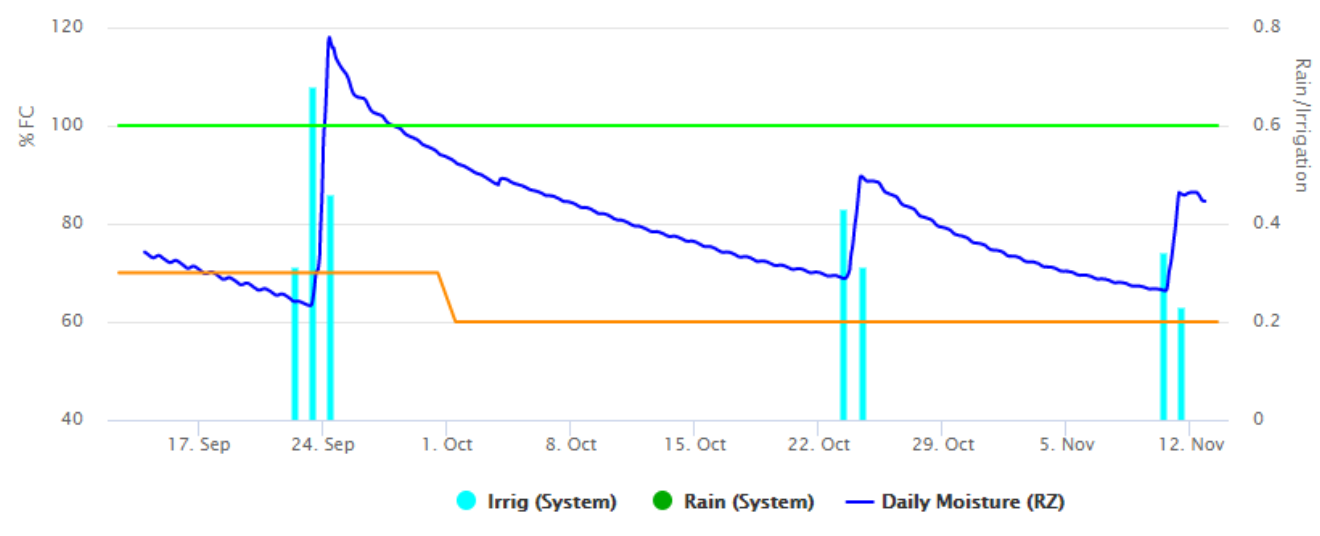
\includegraphics[width=0.6\linewidth]{grafiek.png}
	\caption{\orange{Wat beken die Groen en Oranje Lyne in hierdie grafiek?  Verwys die area onder oranje wanneer die plant stres ervaar?  Dui die groen lyn maar net aan wanneer die Field Capacity 100\% is?}}
\end{figure}

\emph{Die {\kc} kurwe van 'n plant is altyd 'n positief klokvorm en maak nooit sporadiese spikes nie.}\\
\orange{Bestaan die {\kc} kurwe uit die fases:  (i) Initial, (ii) Crop Development, (iii) Mid-Season, (iv) Late-Season.  Is Figure 2 hieronder 'n regte voorbeeld van die {\kc} kurwe?}\\
\begin{figure}[!h]
	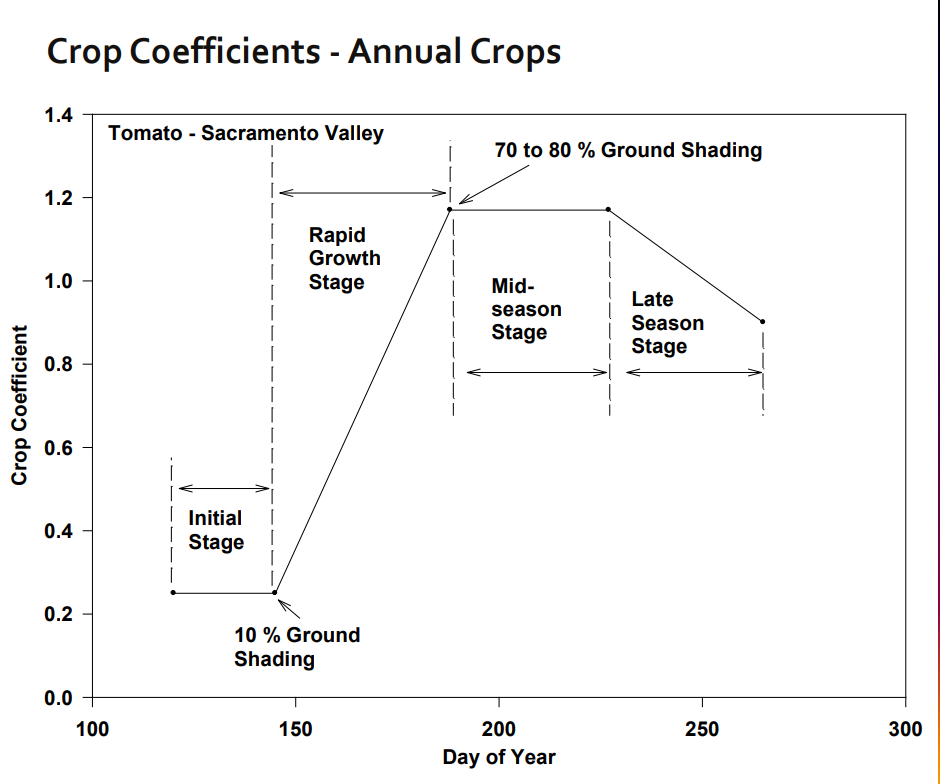
\includegraphics[width=0.5\linewidth]{Kc_curve.png}
	\caption{Voorbeel van {\kc} kurwe as 'n funksie van `Day of the Year'.}
\end{figure}

\emph{Daarom is {\kc} nie direk gekoppel aan datums nie maar wel aan GDD (wat min or meer met datums ooreenstem)}.\\
\orange{Ek stem saam met hierdie stelling, maar wil wel noem dat 'n website genoem het dat: ``The relationship between {\kc} and crop coverage is more universal than other {\kc} relationships...''.  Later in die dokument noem Jac wel dat hy nie data het oor blaarbedekking nie, maar dat dit gekoppel is aan GDD en {\kc}.}

\emph{Trek $\mathrm{ET}_{CP}$, re\"{e}n en besproeiing uit WaterBalans tabel.}\\
\orange{Wat is hierdie WaterBalans tabel en waar word dit gekry?  Genereer PS se sagteware die WaterBalans Tabel?}

\emph{Kyk of probe data volledig is en vul gapings as dit klein is en die interpretasie logies is.}\\
\orange{Is die data wat hierna verwys word die grondvogstatus wat deur probes gemeet word?}

\emph{Vir SA begin GDD berekening by 1 Augustus en word bereken as:}
\begin{equation*}
\mathrm{GDD} = \frac{T_{\mathrm{min}} + T_{\mathrm{max}}}{2} - 10^{\circ}C
\end{equation*}
\orange{Ek neem aan dat die $10^\circ$ die `Temperature Base' is vir Appels waarmee Jac eerste wil begin werk?  (Temperature Base is the temperature below which plant development stops.)}

\emph{Doen herberekenings om die logika te laat werk in VSA se duime.}\\
\orange{Hierdie is maklik:  $1'' = 25.4\,\mathrm{mm}$ en $1\,\mathrm{mm}=0.0393701''$}

\emph{In die agtergrond dokument het jy vir Jac verduidelik:  ``Hieronder is van die veranderlikes wat ek ge\"{i}dentifiseer het want ons kan gebruik''... Onder andere word {\kc}-oorspronklik en {\kc}-aangepas genoem.}\\
\orange{Kan jy asseblief meer spesifiek uitbrei wat is die verskil tussen hierdie twee {\kc}'s.}

\emph{Verder word ``Ander Probe Data'' ook genoem in die lys, en Jac s\^{e} dat hy baie neutron data het wat eenmaal per week gelees word.}\\
\orange{Watter inligting presies verskaf die Neutron data?  Is dit miskien data van Neutron Monitors wat kosmiese strale meet?}

\end{document}